\documentclass{beamer}
\usetheme{Warsaw}

\newenvironment<>{varblock}[2][.9\textwidth]{%
  \setlength{\textwidth}{#1}
  \begin{actionenv}#3%
    \def\insertblocktitle{#2}%
    \par%
    \usebeamertemplate{block begin}}
  {\par%
    \usebeamertemplate{block end}%
  \end{actionenv}}


\title{FreeJDAQ}
\subtitle{Visuelle Programmiersprache zur Datenerfassung auf
einem Raspberry Pi}
\author{David Gawron, Stefan Geretschlaeger, Leon Huck,
Jan Kublbeck, Linus Ruhnke }
\date{23.09.2019}

\begin{document}

\begin{frame}
\titlepage
\end{frame}

\begin{frame}{Einleitung}
\frametitle{Problemstellung}
	\begin{figure}[htbp]
    	\begin{center}
       	 
\includegraphics[width = 5cm]{Grafiken/FreeJDAQ.png}
    	\end{center}
	\end{figure}
\end{frame}

\begin{frame}{Einleitung}
\frametitle{Abgrenzungen}
\end{frame}

\begin{frame}{Softwaretechnik}
\frametitle{Grundaufbau}
\end{frame}

\begin{frame}{Softwaretechnik}
\frametitle{Paketdiagramm}
\end{frame}

\begin{frame}{Statisitken}
\frametitle{Qualitätssicherung}
\end{frame}

\begin{frame}{Statistiken}
\frametitle{Testüberdeckung}
\end{frame}

\begin{frame}{Statistiken}
\frametitle{GitHub- FreeJDaq}
\end{frame}

\begin{frame}{Statistiken}
\frametitle{GitHub- DAQDocuments}
\end{frame}

\begin{frame}{Tools}
\frametitle{Allgemein}

\begin{varblock}[3cm]{UML}
\begin{figure}[htbp]
    	\begin{center}
       	 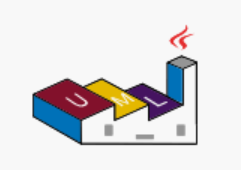
\includegraphics[width = 2cm]{Grafiken/PlantUmlIcon.png}
    	\end{center}
	\end{figure}
\end{varblock}

\begin{varblock}[3cm]{IDE}
\begin{figure}[htbp]
    	\begin{center}
       	 
\includegraphics[width = 2cm]{Grafiken/EclipseIcon.png}
    	\end{center}
	\end{figure}
\end{varblock}

\begin{varblock}[3cm]{Unit-Testing}
\begin{figure}[htbp]
    	\begin{center}
       	 
\includegraphics[width = 2cm]{Grafiken/JUnitIcon.png}
    	\end{center}
	\end{figure}
\end{varblock}

\end{frame}

\begin{frame}{Tools}
\frametitle{Allgemein}

\begin{varblock}[3cm]{Integration}
\begin{figure}[htbp]
    	\begin{center}
       	 
\includegraphics[width = 2cm]{Grafiken/MavenIcon.png}
    	\end{center}
	\end{figure}
\end{varblock}

\begin{varblock}[3cm]{Code-Testing}
\begin{figure}[htbp]
    	\begin{center}
       	 
\includegraphics[width = 2cm]{Grafiken/JacocoIcon.png}
    	\end{center}
	\end{figure}
\end{varblock}

\begin{varblock}[3cm]{Code-Testing}
\begin{figure}[htbp]
    	\begin{center}
       	 
\includegraphics[width = 2cm]{Grafiken/EclEmmaIcon.png}
    	\end{center}
	\end{figure}
\end{varblock}

\end{frame}

\begin{frame}{Tools}
\frametitle{Allgemein}

\begin{varblock}[3cm]{Code-Testing}
\begin{figure}[htbp]
    	\begin{center}
       	 
\includegraphics[width = 2cm]{Grafiken/SonarlintIcon.png}
    	\end{center}
	\end{figure}
\end{varblock}

\begin{varblock}[3cm]{Yaml-Editor}
\begin{figure}[htbp]
    	\begin{center}
       	 
\includegraphics[width = 2cm]{Grafiken/SnakeYamlIcon.png}
    	\end{center}
	\end{figure}
\end{varblock}

\end{frame}

\end{document}